\subsection{\secState{R}Map Obstacles}\label{s:mapObstacles}
\paragraph{Idea:} Use \emph{stored LiDAR readings} from previous mission to build an compact obstacle map \cite{cernamaria2018}. Then use \emph{this map} as a additional information source.

\paragraph{Concept:} A \emph{map obstacle} state has very simple logic, there are three possible cases:

\begin{enumerate}
    \item \emph{Undetected} - Map obstacle $O_M$ is charted on map (fig. \ref{fig:undetectedMapObstalce}), but is undetected by any sensor in sensor field, therefore the probability of map obstacle occurrence is equal to $0$.


    \item \emph{Detected} Map obstacle $O_M$ is charted on map and detected by any sensor in sensor field (fig. \ref{fig:detectedMapObstacle}). The map obstacle rate is equal to detected obstacle rate, usually its equal to $1$.

    \item \emph{Hindered} Map obstacle $O_M$ is hindered behind other detected obstacle $O_1$ (fig. \ref{fig:hinderedMapObstacle}). The detected obstacle $O_1$ is in $cell_{i,j,k}$ and is reducing visibility in follow up $cellRow_{i_f>i,j,k}$ by $60$ percent.
\end{enumerate}

\begin{figure}[H]
    \begin{subfigure}{0.32\textwidth}
        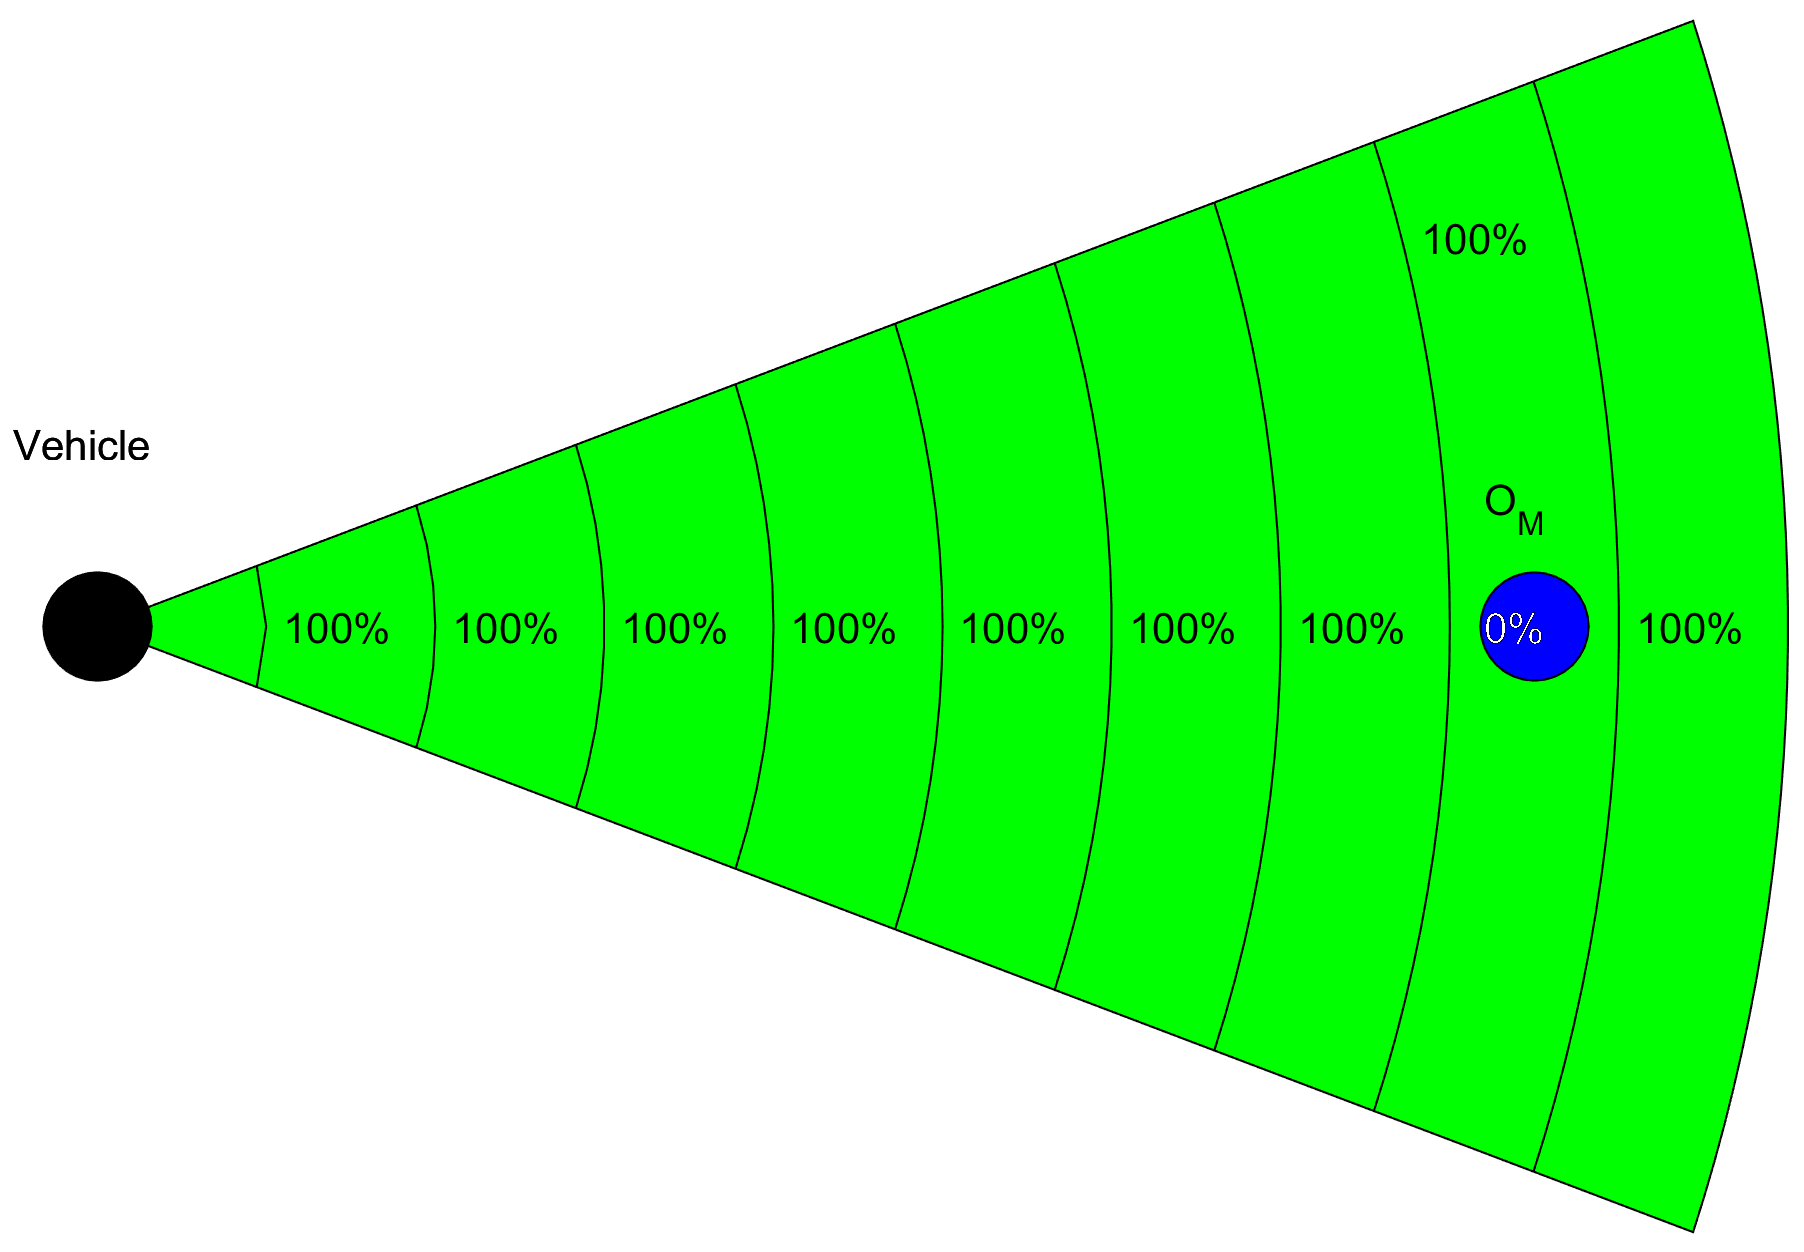
\includegraphics[width=0.9\linewidth]{\FIGDIR/TE009MapObstacleUndetected} 
        \caption{Undetected.}
        \label{fig:undetectedMapObstalce}
    \end{subfigure}
    \begin{subfigure}{0.32\textwidth}
        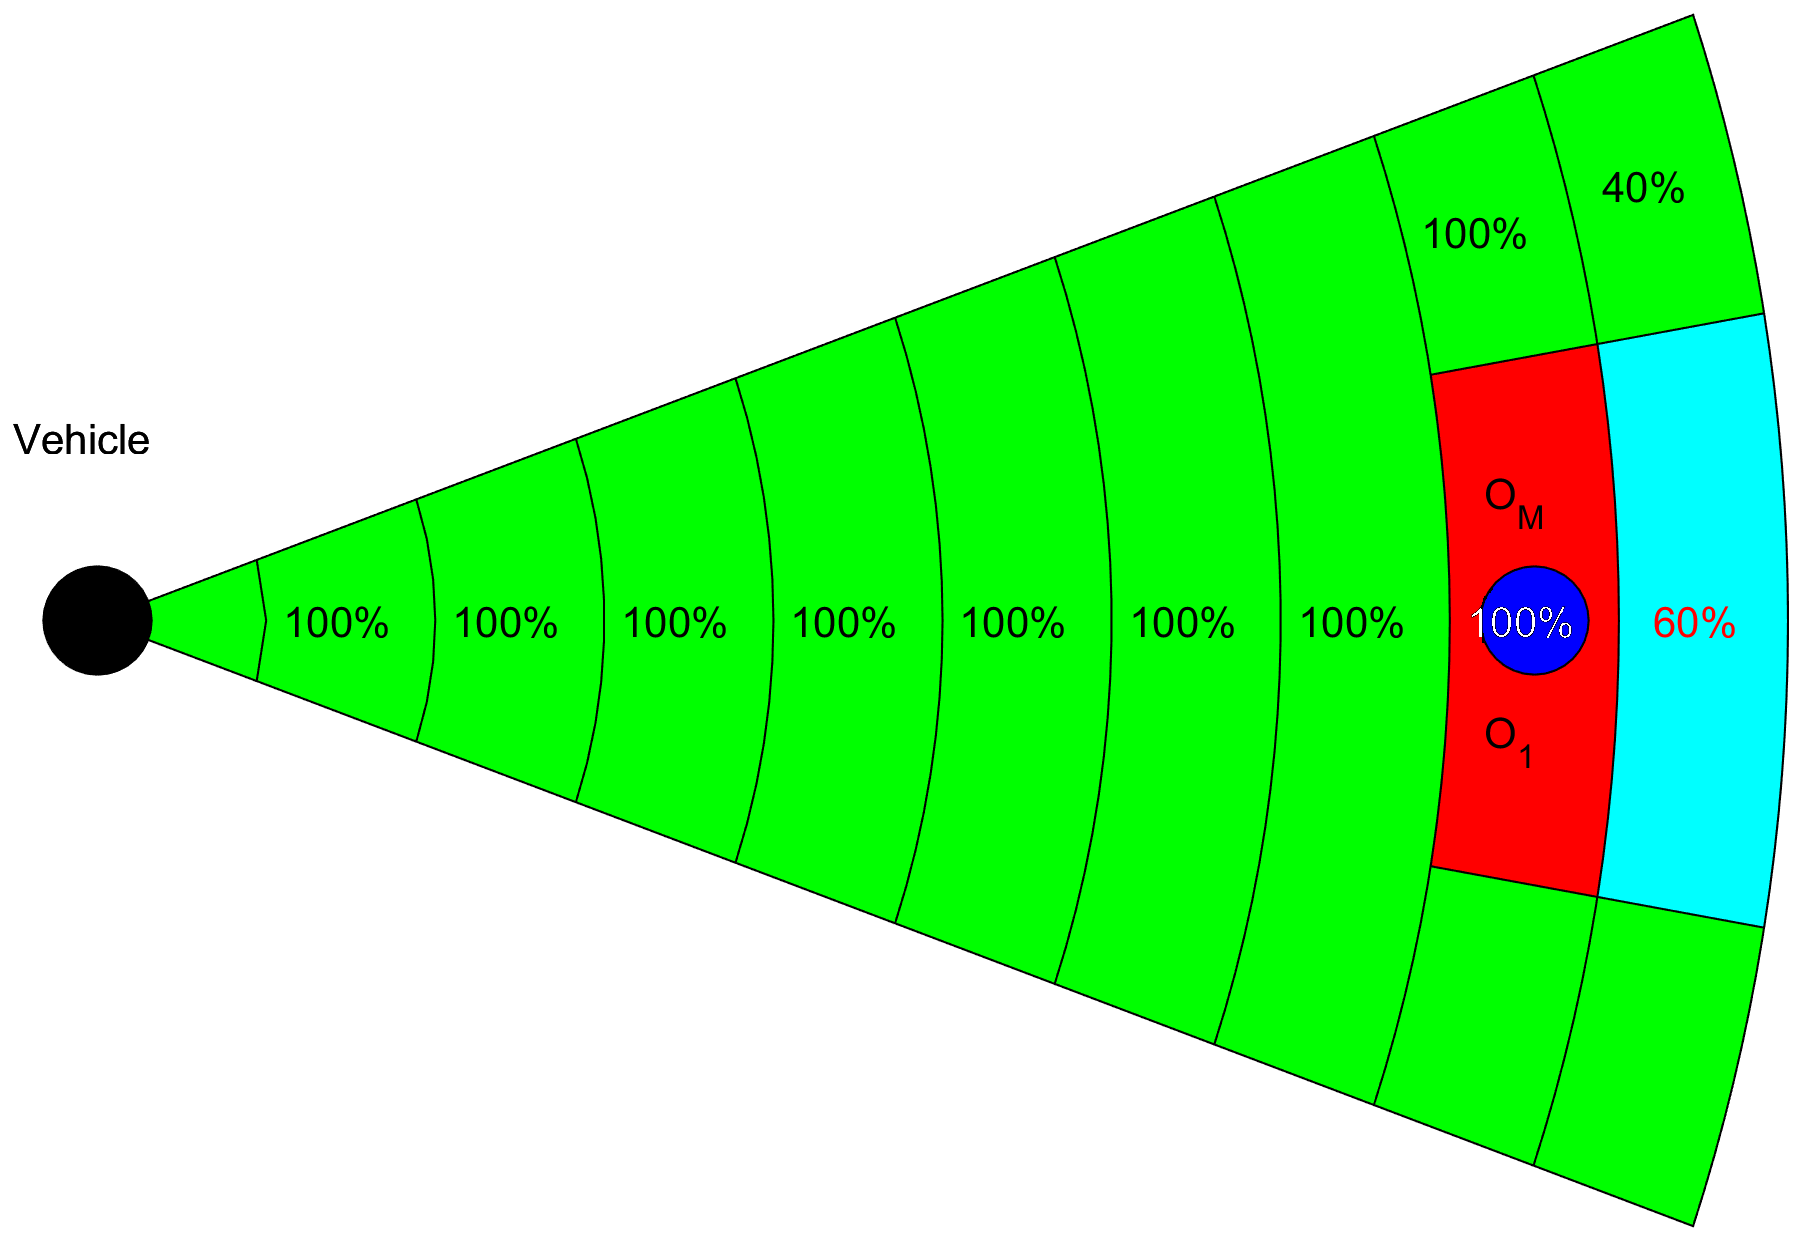
\includegraphics[width=0.9\linewidth]{\FIGDIR/TE010MapObstacleDetected} 
        \caption{Detected.}
        \label{fig:detectedMapObstacle}
    \end{subfigure}
    \begin{subfigure}{0.32\textwidth}
        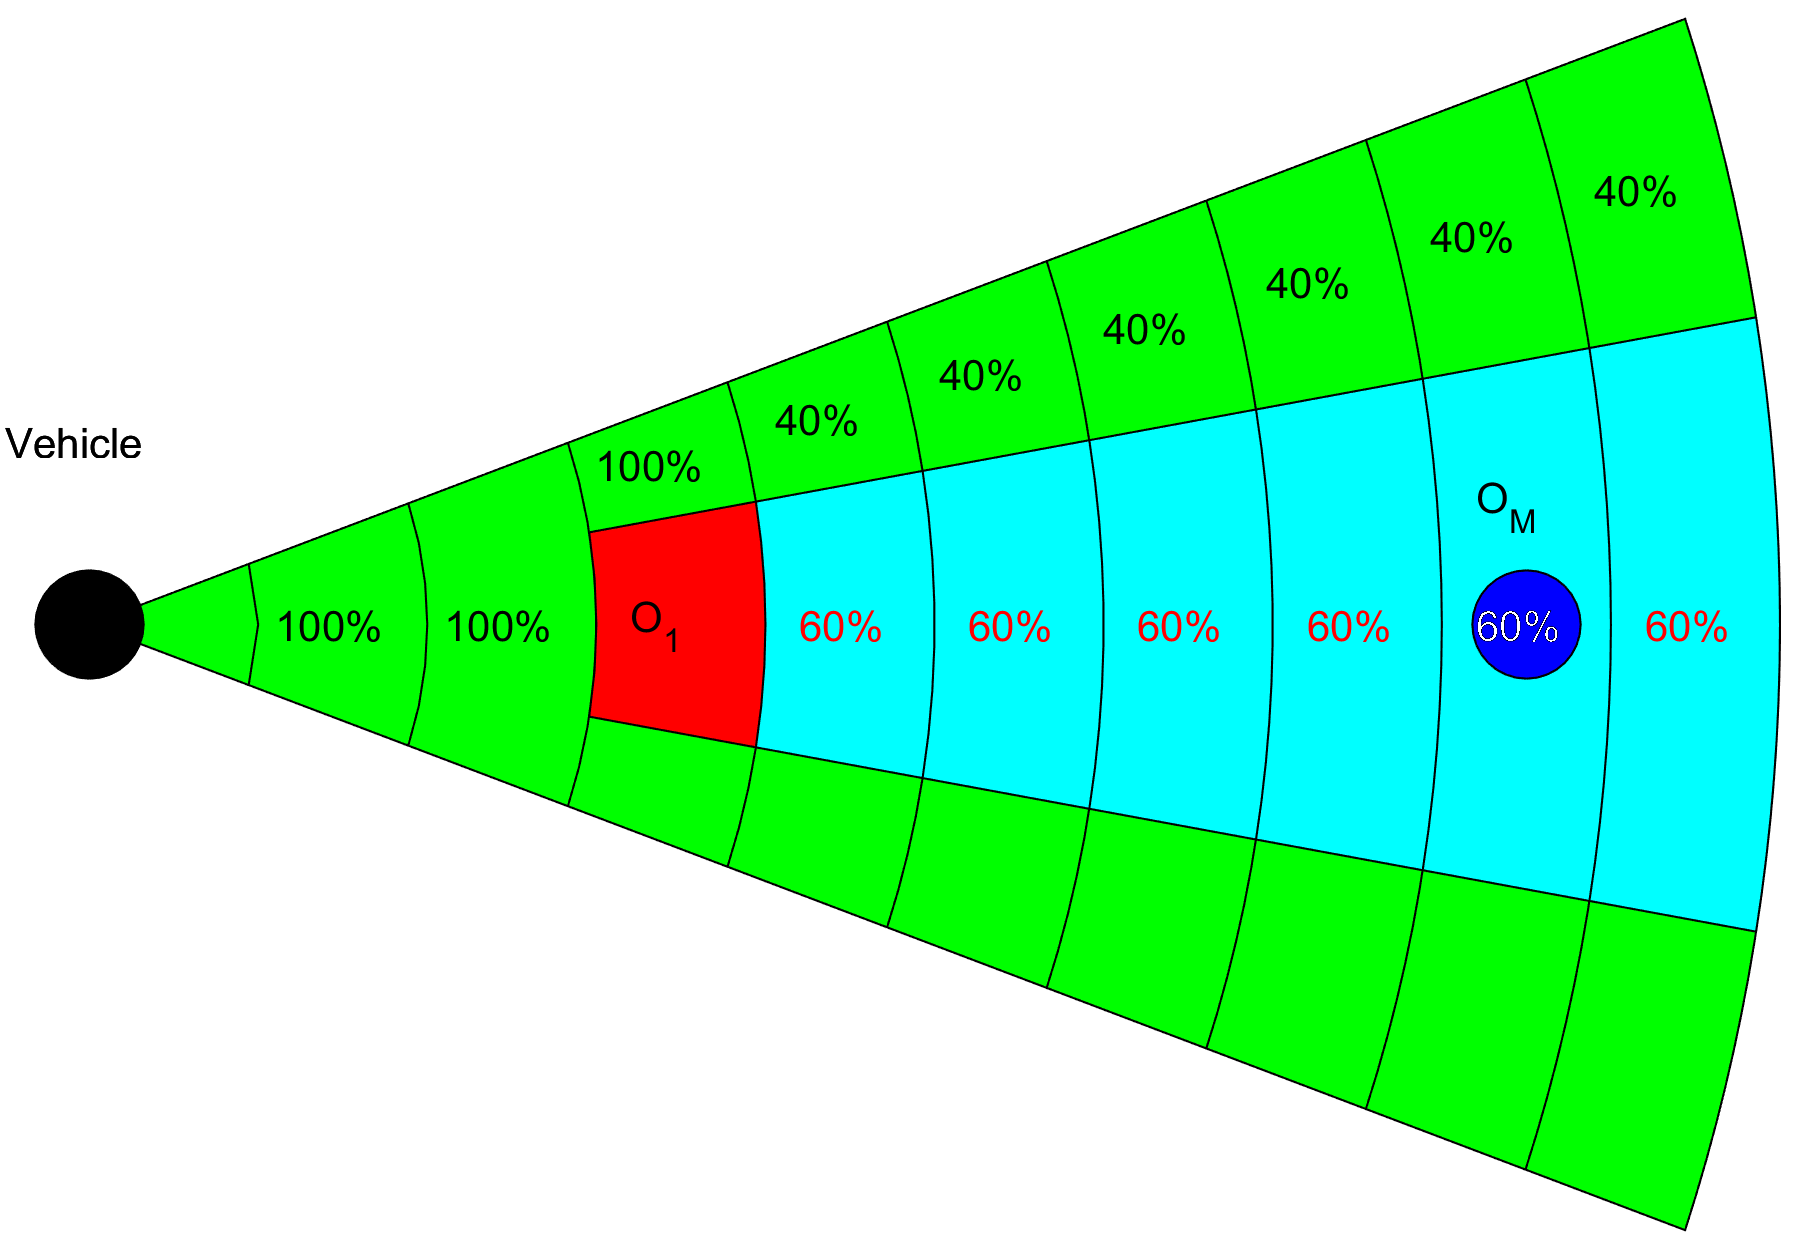
\includegraphics[width=0.9\linewidth]{\FIGDIR/TE011MapObstacleHiden}
        \caption{Hindered.}
        \label{fig:hinderedMapObstacle}
    \end{subfigure}
    \caption{Map obstacle states after \emph{Data fusion}.}
    \label{fig:mapObstacleStatesAfterDataFusion}
\end{figure}

\paragraph{Implementation:} The formulation of final map obstacle rate  $map(cell_{i,j,k})$ was outlined in previous examples. These examples are showing the \emph{desired behaviour} and its solved by \emph{data fusion} (sec. \ref{s:sensorFusion}).

First we start with obstacle map definition. The obstacle map  (eq. \ref{eq:obstacleMap}) defines an map obstacle set of information vectors with position in global coordinate frame , orientation bounded to global coordinate reference frame, safety margin and additional parameters.
\begin{equation}\label{eq:obstacleMap}
    obstacle Map= 
    \left\{
    \begin{bmatrix}
        position,\\
        orientation,\\
        safety Margin,\\
        parameters
    \end{bmatrix}
    :
    \begin{aligned}
        & position \in  \R^3(GCF),\\
        & orientation \in \R^3(GCF),\\
        & safety Margin \in \R^+(m),\\
        & parameters \in \{\dots\}
    \end{aligned}
    \right\}
\end{equation}


The \emph{Map Obstacle} concept is taken from my \emph{master student work} \cite{cernamaria2018}, implementing \emph{compact representation} of point-cloud obstacle map. Te example of \emph{cuboid obstacles} with \emph{safe zone} is given in (fig. \ref{fig:exampleExtractedMapObstacles}).
    
\begin{figure}[H]
    \centering
    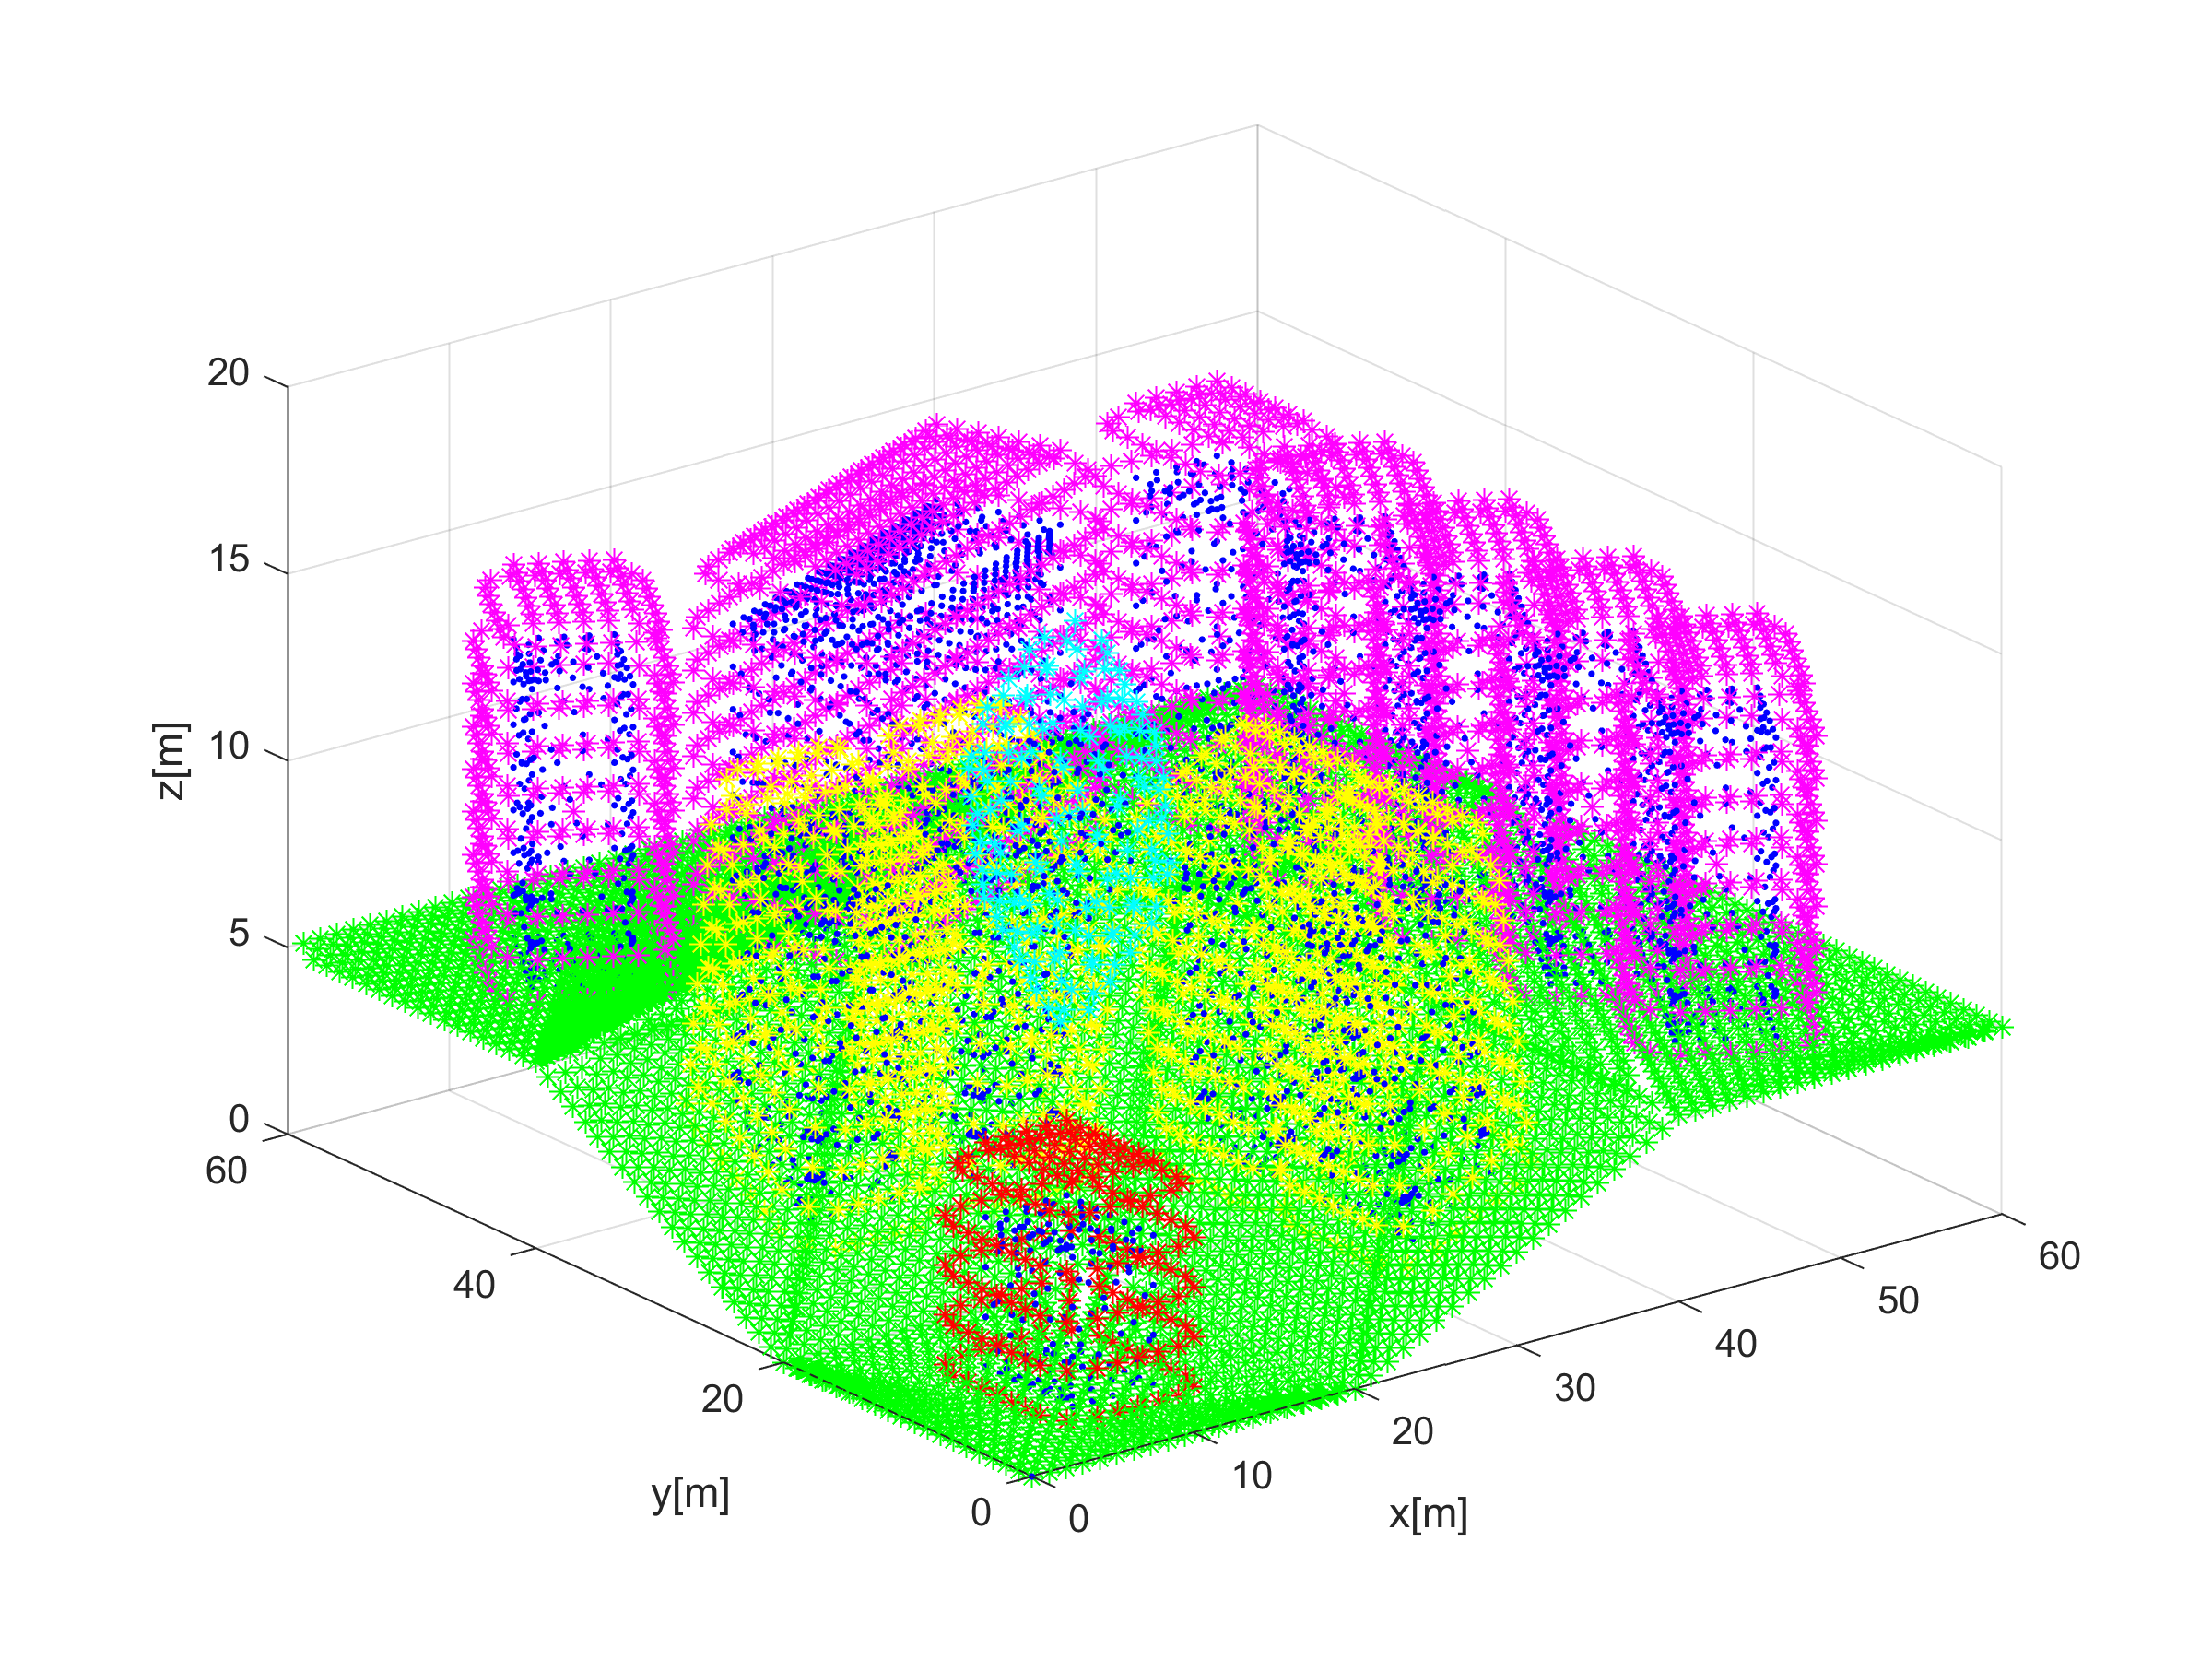
\includegraphics[width=0.7\textwidth]{\FIGDIR/TE054ExtractedMapObstaclesExample}
    \caption{Example of Extracted Map Obstacle \cite{cernamaria2018}.}
    \label{fig:exampleExtractedMapObstacles}
\end{figure} 

\noindent The space covered by any obstacle  is non-empty by definition. There are following types of map charted obstacles which are implemented in framework:

\begin{enumerate}
    \item\emph{Ball obstacle $parameters=\varnothing$} - simple ball with center at $position$, with offset safety margin.
    
    \item\emph{Line obstacle $parameters=[length]$} - simple line bounded by length $\in]0,\infty[$ with center at $position$ and given orientation with respect to main axis in global coordinate frame, with safety margin $<$ 0.
    
    \item\emph{Plane obstacle $parameters=[length,width]$} - bounded rectangle plane partition defined by length $\in]0,\infty[$, and width $w\in]0,\infty[$ with center at $\vec{p}$ and given orientation $\vec{o}$ with respect to main axis in global coordinate frame, with safety margin.
    
    \item\emph{Cuboid obstacle $parameters=[length,width,depth]$} - bounded cuboid space partition defined by length $\in]0,\infty[$, width $\in]0,\infty[$, and depth $d\in]0,\infty[$ with center at $position$ and rotated in orientation with respect to main axis in global coordinate frame, with safety margin.
\end{enumerate}

\noindent The \emph{map obstacles} are stored in clustered database. The \emph{selection criterion} is given in (eq. \ref{eq:mapObstacleSelectionCriterion}).

\begin{equation}\label{eq:mapObstacleSelectionCriterion}
    avoidance Grid.radius \ge distance(UAS.position,map Obstacle) - total Margin
\end{equation}

\noindent The \emph{total margin} is combination of \emph{safety margin} and \emph{body margin} (in case of line, plane, cuboid obstacle). The \emph{selection} was implemented as standard cluster select, selecting 26  surrounding clusters around UAS + own UAS cluster.

The \emph{compact obstacle representation} is transformed into \emph homogeneous point-cloud representations:

\begin{itemize}
    \item[1.]\emph{Body Point-cloud} - representing obstacle body approximation by geometrical shape (eq. \ref{eq:mapBodyPointCloud}). This point cloud is considered as hard constraints.
    
    \begin{equation}\label{eq:mapBodyPointCloud}
        body Point Cloud  =\{point\in\R^3(GCF): point \in map Obstacle Body\}
    \end{equation}
    
    \item[2.]\emph{Safety Margin Point Cloud} - representing safety coating around mapped obstacle body approximation (eq. \ref{eq:mapMarginPointCloud}). This point cloud is considered as soft constraint.
    \begin{equation}\label{eq:mapMarginPointCloud}
        margin Point Cloud = \{point\in\R^3(GCF): point \in map Safety Margin\}
    \end{equation}
\end{itemize}

\begin{note}
    The \emph{safety margin point cloud} is hollow in relationship to an \emph{body point cloud}, therefore:
    \begin{equation*}
        body Point Cloud \cap margin Point Cloud  = \varnothing
    \end{equation*}
\end{note}

\noindent The \emph{map obstacle} discretization to point cloud leads to problem how to calculate \emph{impact rate}. The \emph{theoretical impact rate} for \emph{obstacle} is given as:
\begin{equation*}
    impact Rate = \frac{volume(map Obstacle\cap cell_{i,j,k})}{volume(cell_{i,j,k})}\in [0,1]
\end{equation*}

\noindent The \emph{map obstacle related point clouds} (eq. \ref{eq:mapBodyPointCloud}, \ref{eq:mapMarginPointCloud}) are homogeneous \cite{cernamaria2018}. That means \emph{each point} in point clouds covers similar portion of object volume. There is \emph{threshold volume} (eq. \ref{eq:tresholdVolumeDefinition}) which represents minimal object volume to be considered as an \emph{obstacle}.

\begin{equation}\label{eq:tresholdVolumeDefinition}
    0< threshold Volume \le \frac{volume(point Cloud)}{|point Cloud|}
\end{equation}

\noindent The \emph{impact rate} of one point  when intersecting a $cell_{i,j,k}$ is given as count of \emph{threshold obstacle bodies} in \emph{point cloud covered mass} multiplied by inverted point count (eq. \ref{eq:pointImpactRateMap}).

\begin{equation}\label{eq:pointImpactRateMap}
    point. rate = \frac{point Cloud Volume}{threshold Volume}\times\frac{1}{|point Cloud|}
\end{equation}

The \emph{intersection set} between \emph{point cloud} and $cell_{i,j,k}$ is defined in (eq. \ref{eq:pointImpactRateMap}). The \emph{cell} intersection with points is defined in (eq. \ref{eq:boundedSpaceCell}).

\begin{multline}\label{eq:pointcloudIntersectionMap}
    intersection(map,cell_{i,j,k}) =\dots\\\dots \{points \in \R^3: (point\to Avoidance Grid Frame) \in cell_{i,j,k}\}
\end{multline}

\noindent The \emph{map obstacle rating} for $cell_{i,j,k}$ and obstacle for our \emph{information source} is defined in (eq. \ref{eq:mapcellratingourMap}).

\begin{equation}\label{eq:mapcellratingourMap}
    map(cell_{i,j,k},obstacle) =\max\left\{ \sum_{\forall point\in intersection(map,cell_{i,j,k})}  point.rate , 1\right\}
\end{equation}

\noindent The \emph{map obstacle rating} for $cell_{i,j,k}$ and \emph{our information source} is given as maximum of all possible cumulative ratings form each obstacle in \emph{active map obstacles} set (eq. \ref{eq:cumulativeMapCellRatingMap}).

\begin{equation}\label{eq:cumulativeMapCellRatingMap}
    map(cell_{i,j,k} = \max \left\{map(cell_{i,j,k},obstacle):\forall obstacle \in Active Map Obstacles\right\}
\end{equation}

\begin{note}
    The \emph{body point clouds} (eq. \ref{eq:mapBodyPointCloud}) never intersects, because they are created for inclusive obstacles. The \emph{safety margin point clouds} (eq. \ref{eq:mapMarginPointCloud}) can intersects, because they represents protection zones around physical obstacles. Therefore the \emph{maximum obstacle rating} (eq. \ref{eq:cumulativeMapCellRatingMap}) needs to be selected.
\end{note}
